\chapter{Use Cases} \label{chap:usecases}
To evaluate our approach, we have implemented the general method described in the previous sections as a C++ class integrated with a research toolset used for designing and testing different conventional DGGSs.
In this toolset, the operations provided by a DGGS are specified by an abstract class that each implementation extends.
The 3D DGGS class takes an input DGGS as well as values for the target aspect ratio ($a$), exponent for the radial mapping ($t$), and the radial range of the grid ($R_\mathrm{max}$ and $R_\mathrm{min}$) as input during construction.
The 3D DGGS uses these values---along with the operations and information provided by the input DGGS---to provide the functionality described in the paper: point encoding, cell decoding, parents, children, and neighbours.
We also provide the ability to create basic visualization of the grid.
These visualizations were used as a basis for many of the figures in this paper.


We evaluate our system by looking at three sample use cases for our 3D DGGSs.
These use cases are not meant to be state-of-the-art implementations of a 3D global grid system, but rather are meant to demonstrate the robustness and versatility of the approach and its ability to support different target applications, data sets, and input DGGSs.
For each use case, we chose an input DGGS and parameters for the system that resulted in a 3D DGGS with desirable properties for said application.
The data encodings in these use cases are all defined using the fundamental operations of the 3D DGGS listed above.


\section{Aircraft and Satellite Paths}
The first use case we examine is tracking the trajectories of aircraft and spacecraft, such as commercial and private flights, drones, satellites, and rockets.
Such a system could be used to increase the efficiency of collision queries using the hierarchy of the grid system, similar to the approaches of~~\cite{miao2019low, zhai2019collision}.
The main benefit our 3D DGGS would offer over existing grids for such a system is the ability to have cells located at low and high altitudes in the same resolution have close to equal shape and size.


\begin{figure}[h]
	\centering
	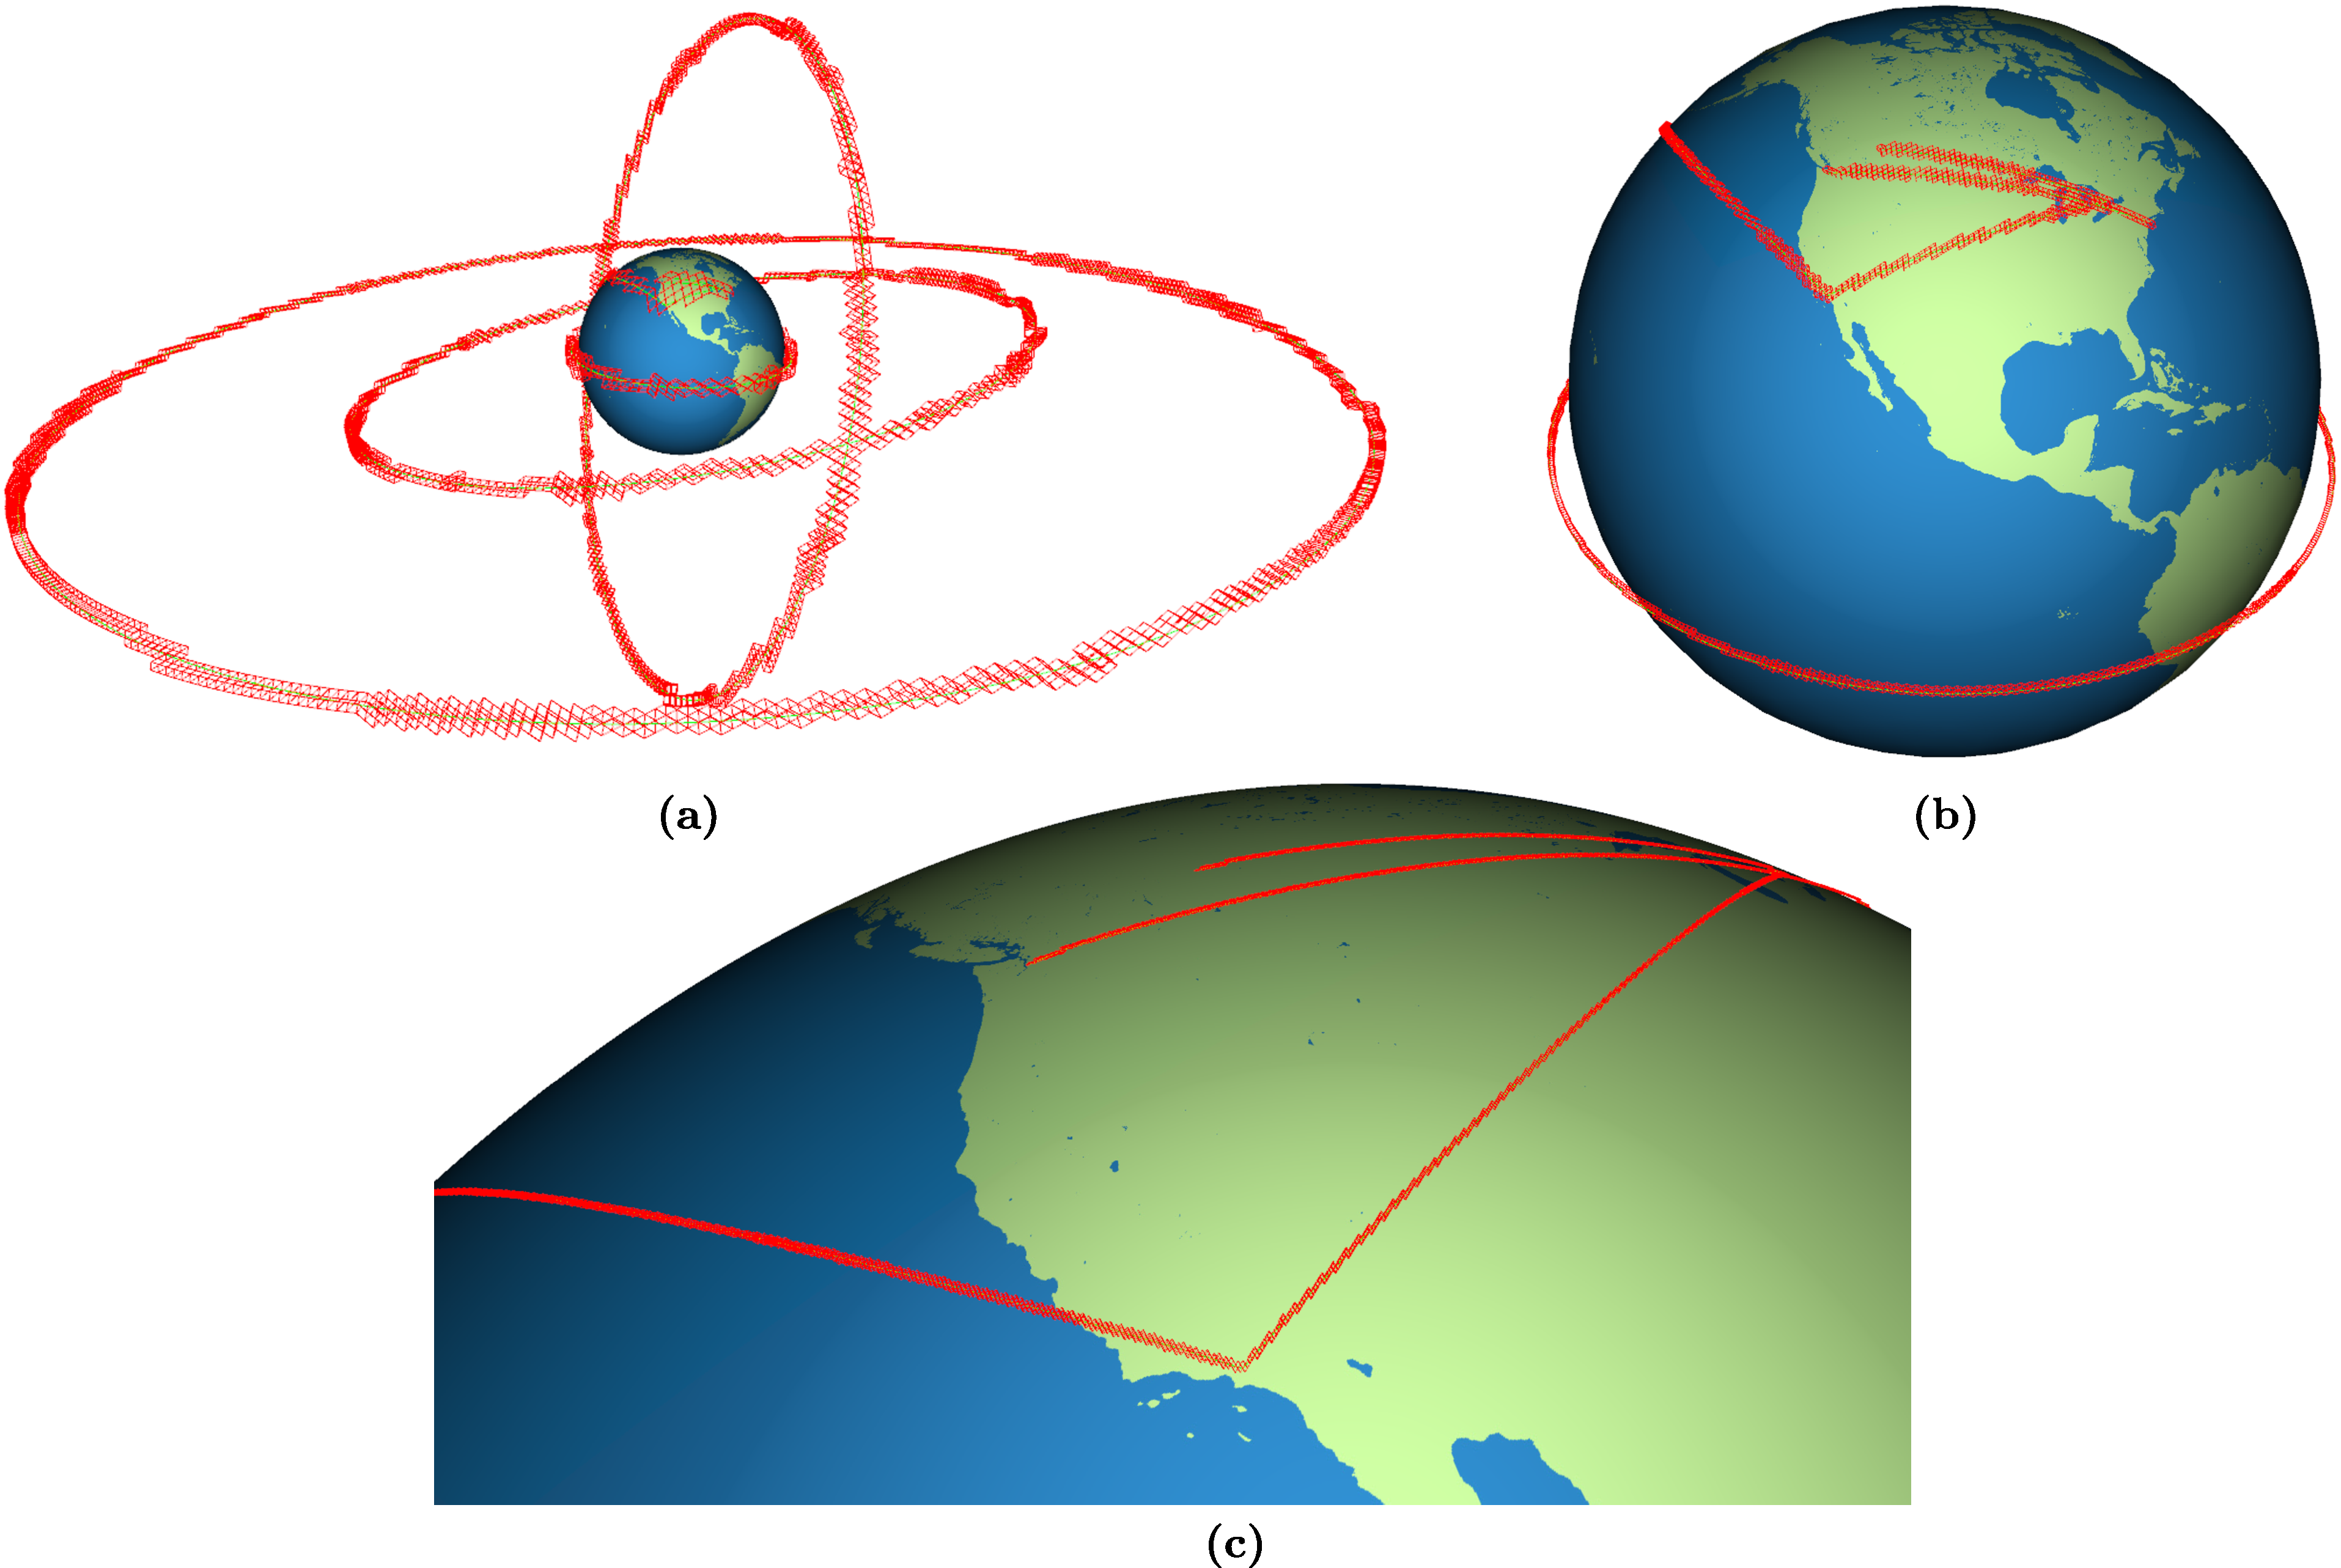
\includegraphics[width=\columnwidth]{satellites.pdf}
	\caption{Flight paths and satellite orbits rasterized in a 3D DGGS.
		All paths and orbits are rasterized at the same grid resolution of \textbf{(a)} 7, \textbf{(b)} 10, and \textbf{(c)} 13}
	\label{fig:satellites}
\end{figure}


Figure~\ref{fig:satellites} shows several generated flight paths and satellite orbits represented in a 3D DGGS at increasing resolutions.
The input DGGS for this example uses a rhombic triacontahedron as the initial polyhedron, standard 1:4 quadrilateral refinement, and a simple normalization projection.
The 3D DGGS has a target aspect ratio of one, a radial mapping exponent of one, and a radial range of 10.66$R$ (67,957~km).
These parameters were chosen to ensure that cells are as compact as possible.

\section{Urban Planning}
The second use case is a volume-preserving 3D grid for the purpose of urban planning and management.
A volume-preserving grid is useful for quickly estimating the volume of a feature that has been rasterized in the grid by multiplying the number of cells by their volume.
This use case also shows the ability of our 3D DGGS to handle small scale data in addition to the much larger scale data showcased in the previous one.


\begin{figure}[h]
	\centering
	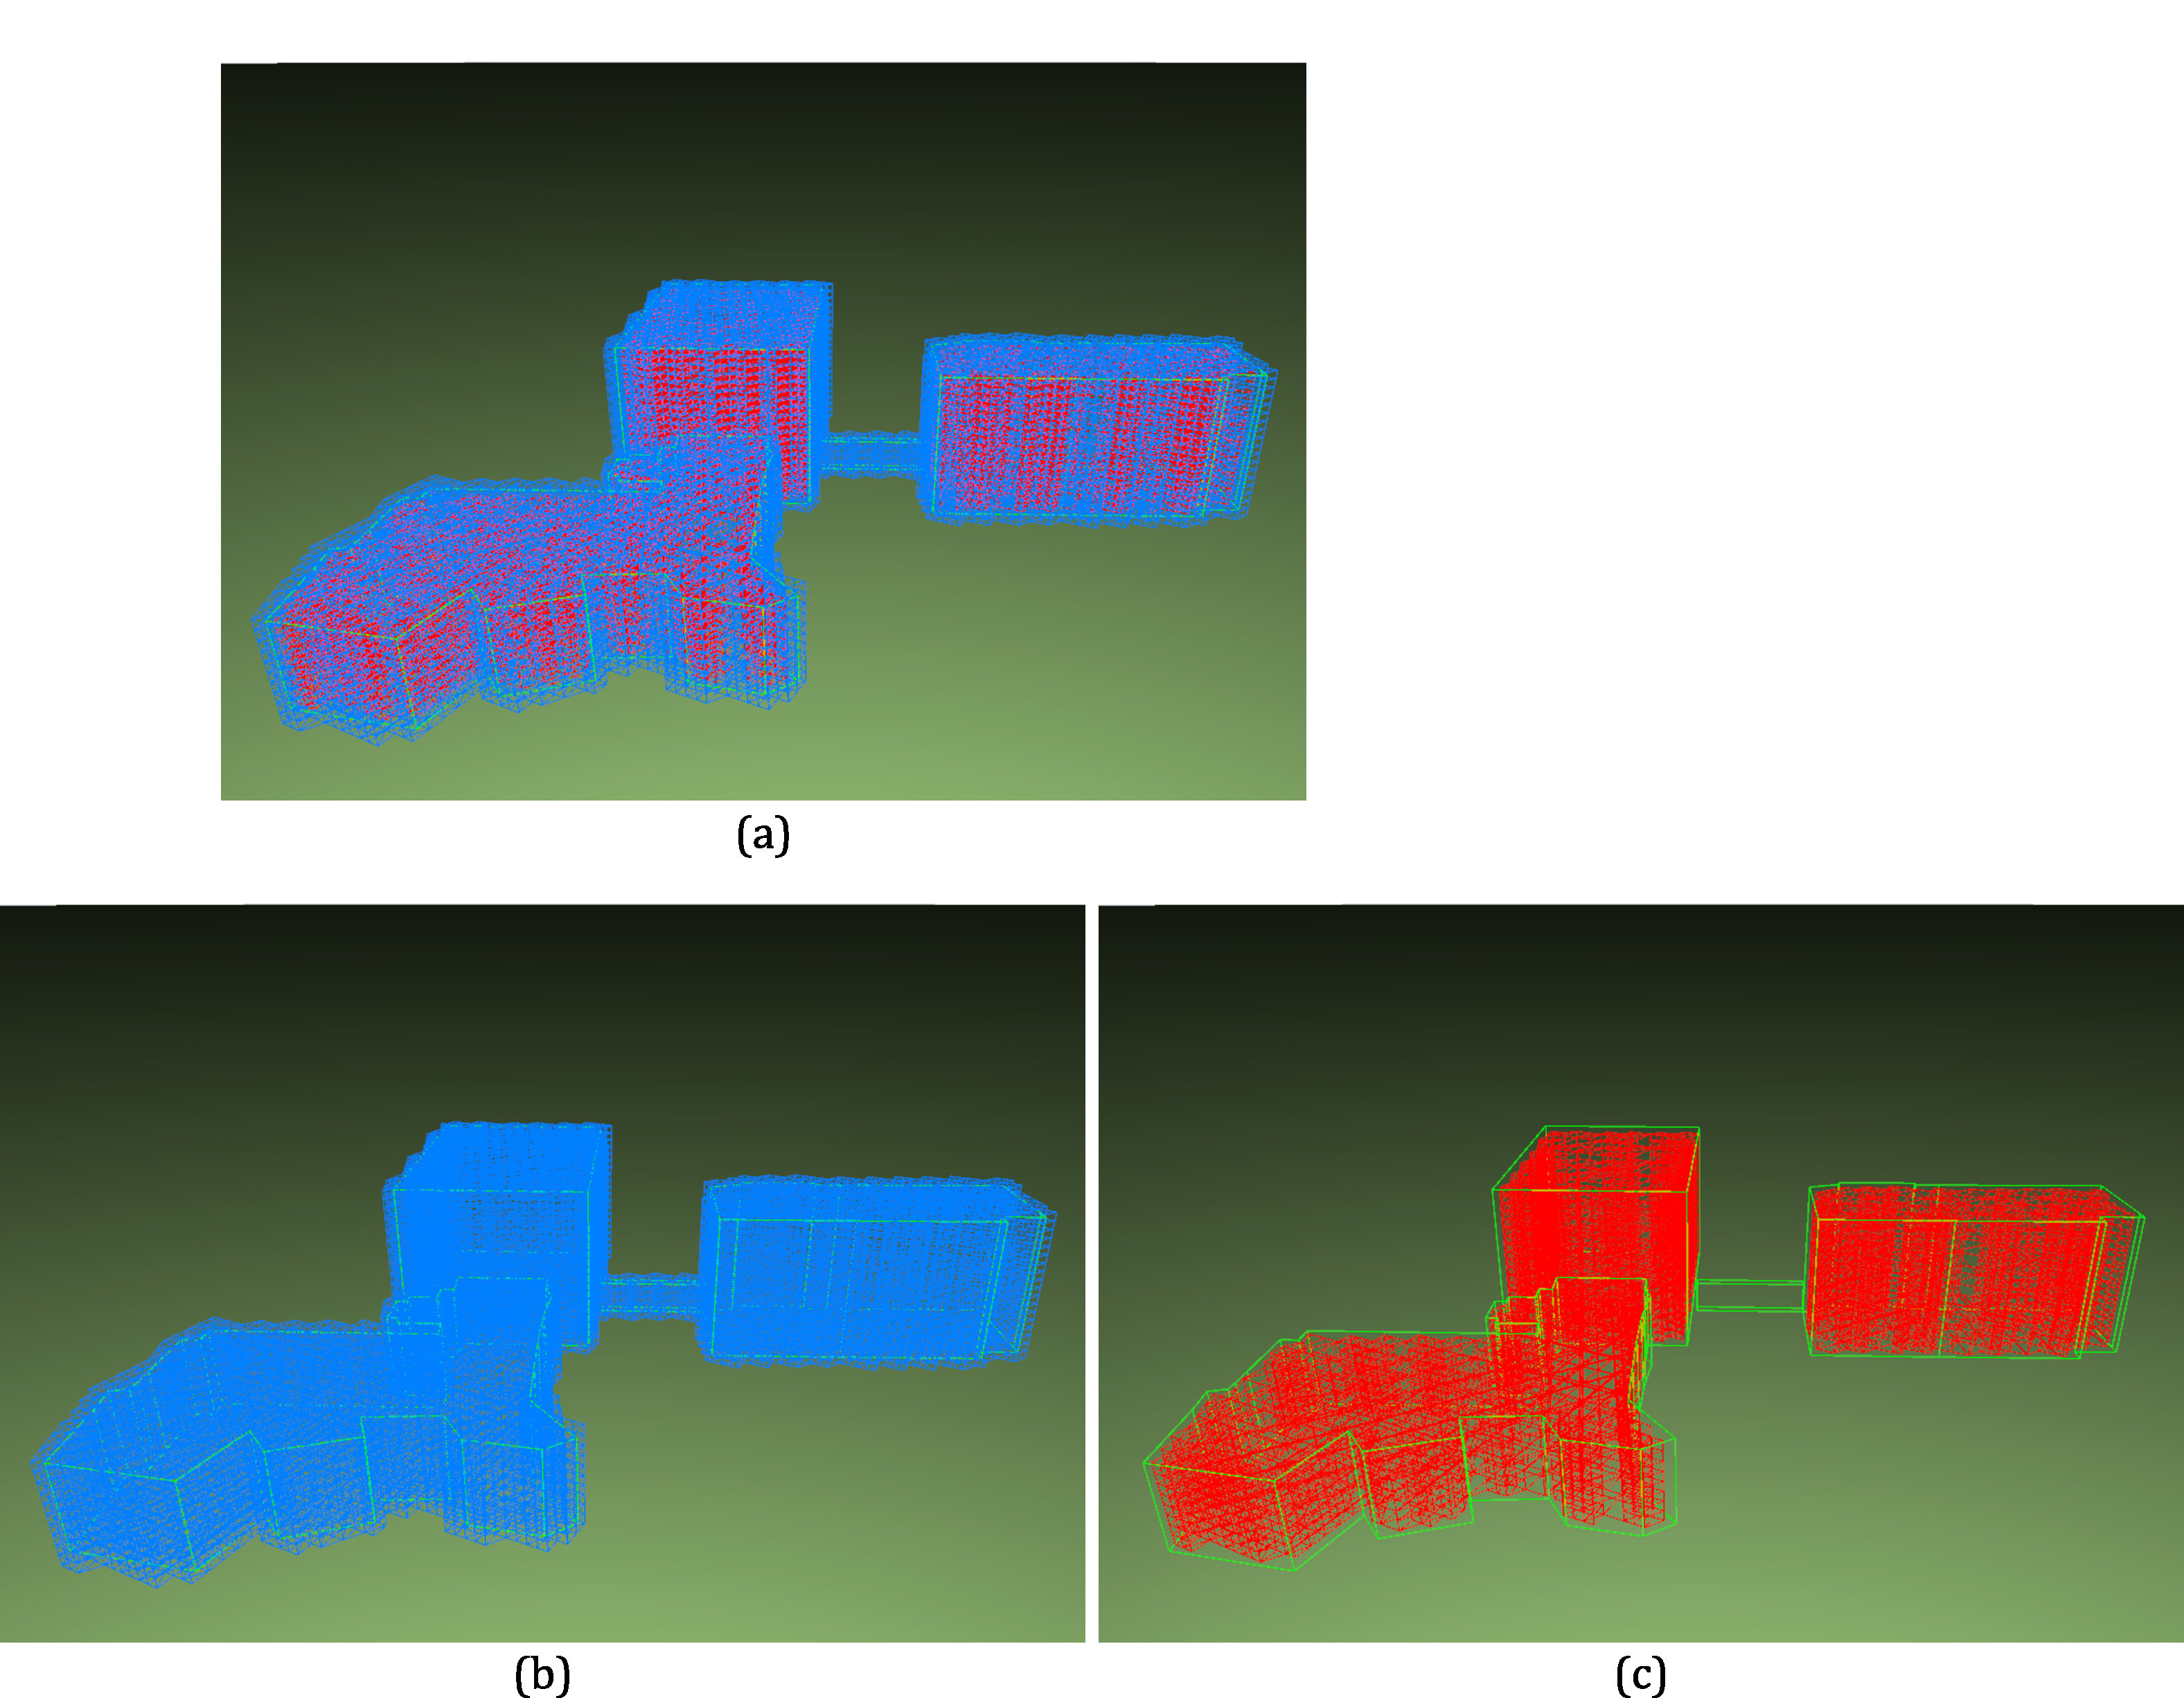
\includegraphics[width=\columnwidth]{buildings.pdf}
	\caption{A collection of buildings from the University of Calgary rasterized in a 3D DGGS at resolution 21.
		In \textbf{(a)}, both interior and boundary cells are shown, whereas \textbf{(b)} and \textbf{(c)} show only boundary and interior cells, respectively}
	\label{fig:urbanplanning}
\end{figure}


Figure~\ref{fig:urbanplanning} shows several buildings represented in a 3D DGGS, with the building geometries obtained from Open Street Map\footnote{\url{www.openstreetmap.org}}.
The input DGGS for this example uses a disdyakis triacontahedron as the initial polyhedron, a non-standard 1:4 triangle refinement to maintain the relative shape of triangles, and the vertex oriented great circle slice and dice projection~\cite{van2006slice} to preserve area~\cite{hallDT}.
The 3D DGGS has a target aspect ratio of one, a radial mapping exponent of three to achieve perfect volume preservation (excluding the central layer), and a maximum radius of 1.33$R$ (8495~km).


\section{Atmospheric Properties}
The final use case we look at is using a 3D DGGS to resample atmospheric forecasts, such as those generated by numerical weather prediction models.
These datasets typically have a much higher vertical resolution than surface resolution, due to how quickly properties such as temperature and wind speed tend to change in these two dimensions.
To accommodate this with our 3D DGGS, we can specify an appropriate aspect ratio for cells to ensure the vertical and surface resolution matches as closely as possible that of the input data.


\begin{figure}[h]
	\centering
	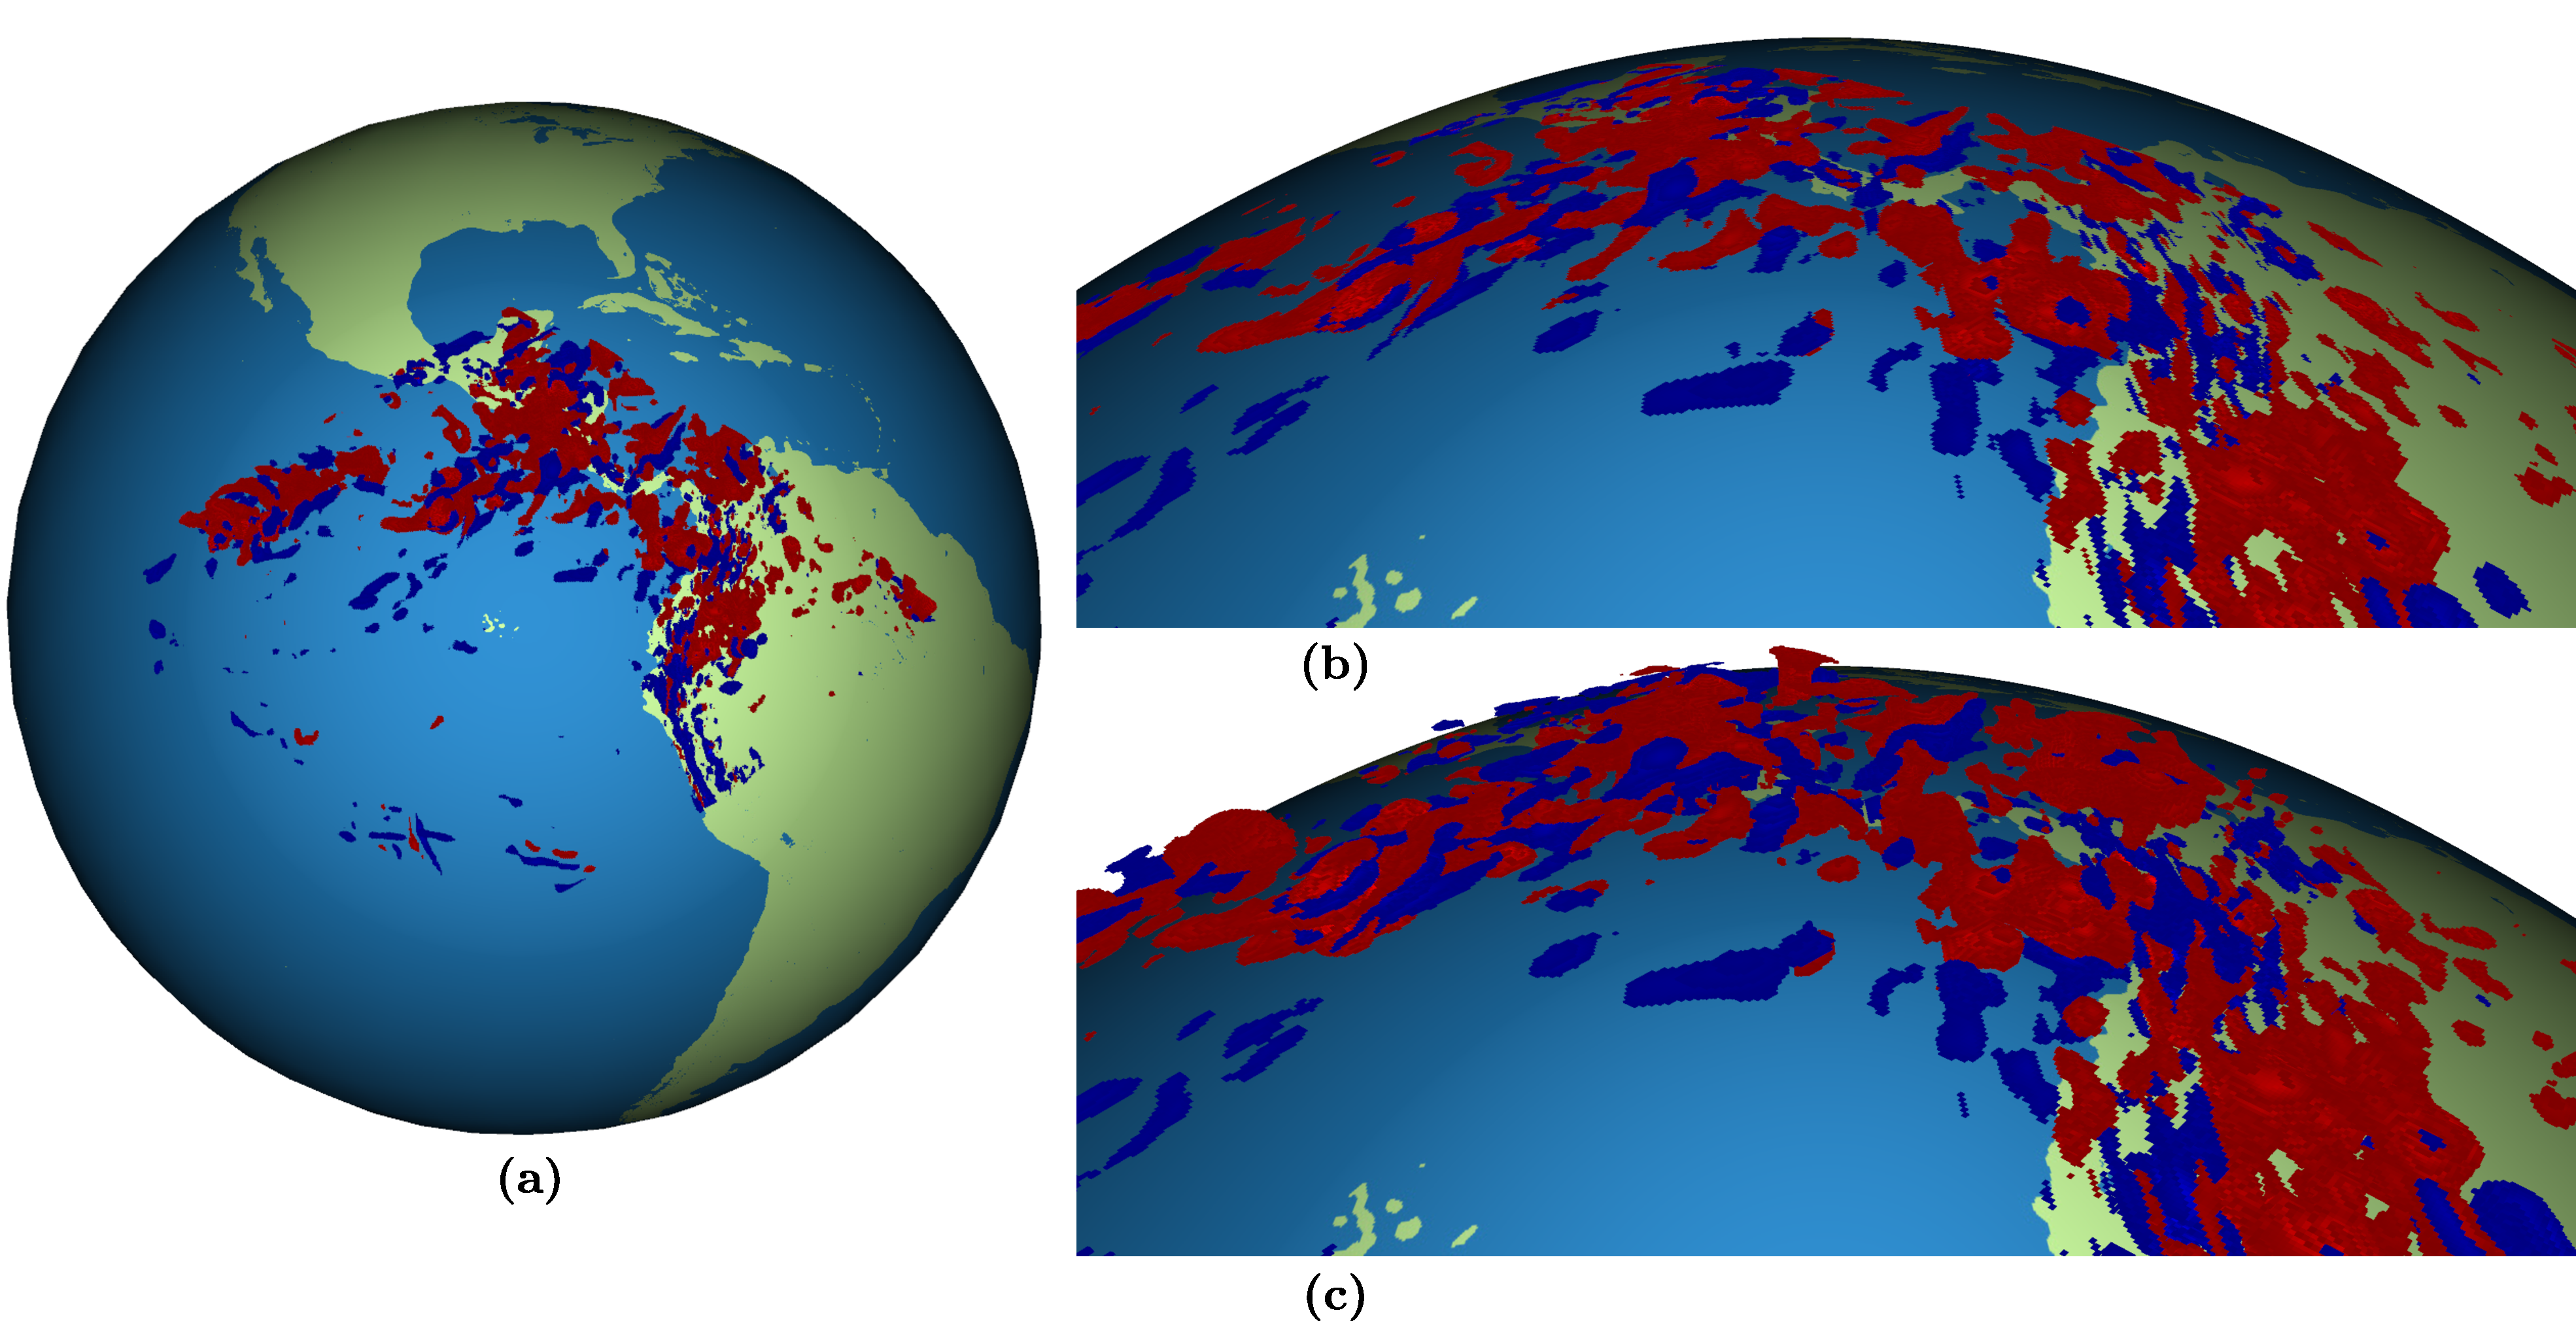
\includegraphics[width=\columnwidth]{atmosphere.pdf}
	\caption{Vertical wind speed (mbar/s) sampled into a 3D DGGS at resolution 9.
		Negative velocity, which corresponds to an upward wind, is shown in red.
		Positive velocity, which corresponds to a downward wind, is shown in blue.
		Velocities with magnitude less than 0.25 mbars/s are not shown to reduce clutter and highlight regions with the highest speeds.
		In \textbf{(a)} and \textbf{(c)}, the altitude of cells is scaled by a factor of 15 to better show changes in altitude.
		In \textbf{(b)}, altitude is shown at its true scale}
	\label{fig:atmosphere}
\end{figure}


Figure~\ref{fig:atmosphere} shows vertical wind speed from the ERA5 dataset~\cite{era5} sampled into a 3D DGGS.
The input DGGS for this example is the same as the one used for the aircraft and satellite paths.
However, this 3D DGGS has a target aspect ratio of 31.7, a radial mapping exponent of one, and a maximum radius of 1.33$R$ (8495~km).


\subsection{Discussion}
The above examples are only a small subset of the many potential applications of our 3D DGGSs.
Despite this, they show not only the useful properties achievable by the method (support for large ranges of altitudes, volume preservation between cells, custom cell aspect ratio, and support for multiple scales of data) but also demonstrate the ease at which new 3D global grids can be created.
Given a conventional DGGS that provides the required operations, creating a 3D DGGS is as simple as providing the surface grid and four clearly defined parameters for the 3D one.
Since creating a 3D DGGS that is ideal for every application is not possible, this allows quick iterations on creating and comparing different 3D grids to find the ideal one for each application.